%!TEX root = ../thesis_phd.tex
%%%%%%%%%%%%%%%%%%%%%%%%%%%%%%%%%%%%%%%%%%%%%%%%%%%%%%%%%%%%%%%%%%%%%%%%%%%%%%%%
%nuosc.tex: Chapter on neutrino physics:
%%%%%%%%%%%%%%%%%%%%%%%%%%%%%%%%%%%%%%%%%%%%%%%%%%%%%%%%%%%%%%%%%%%%%%%%%%%%%%%%
\chapter{Neutrino Oscillations}
\label{nu_osc_chapter}
%%%%%%%%%%%%%%%%%%%%%%%%%%%%%%%%%%%%%%%%%%%%%%%%%%%%%%%%%%%%%%%%%%%%%%%%%%%%%%%%


\section{A Straightforward Interpretation}

Neutrinos are neutral to both the electromagnetic and strong forces.  The effects of gravity are too minute to observe at the energy scales encountered in neutrino experiments.  Therefore, of the four fundamental forces,\footnote{All physical interactions are thought to be mediated by one of four forces: the electromagnetic, strong, weak and gravitational forces.} we only observe neutrinos interacting through the weak force.  When a neutrino interacts, it does so in one of its three weak flavor states: \nue, \numu or $\nu_\tau$.  But in contrast to our intuition, the flavor states do not have definite mass; each is a mixture of three components with distinct masses: $\nu_1$, $\nu_2$ and $\nu_3$.    A neutrino produced in a particular flavor state--- for instance, an electron neutrino produced in the sun--- is composed of some fraction of $\nu_1$, a different fraction of $\nu_2$ and yet another fraction of $\nu_3$.  The mass components propagate as three distinct waves, summing together to make a total wave that is the neutrino.  As these waves travel through space, they move in and out of phase with each other to cause interference; as a result, the composition fractions of the neutrino change.  For every composition of $\nu_1$, $\nu_2$ and $\nu_3$, there are distinct probabilities of interacting as \nue, \numu or $\nu_\tau$.   Thus, when a neutrino reaches its interaction point--- say, the solar neutrino arriving at Homestake mine--- its makeup will have changed to something that may be more likely to interact as a different flavor.   The theory that describes this phenomenon is that of neutrino oscillations.  

\section{Oscillations in Vacuum}

The weak flavor states are the eigenstates of the weak Hamiltonian that governs the neutrino interactions we observe.  A neutrino produced as flavor $l = e, \mu, \tau$ can be written as a superposition of mass states $\alpha = 1, 2, 3$ in terms of the elements of a unitary $3\times3$ matrix $U_{l\alpha}$ as follows:
\begin{equation}\label{superpos}
|\nu_l(0) \rangle = \sum_{\alpha = 1,}^3 U_{l\alpha}|\nu_\alpha(0) \rangle
\end{equation} %check this, should it be U*?
This superposition describes a change of basis and can be likened to rotations in a three dimensional space.   $U_{l\alpha}$ can be written in terms of Euler angles \thetaot, \thetatth and \thetaoth.  In the case rotations in a real vector spaces the matrix would be real; however, for the case of neutrino oscillations we include a complex phase, $\delta$, to allow for the possibility of CP violation.  The matrix U (written here with $c_{ij}$ and $s_{ij}$ as shorthand for $\cos{\theta_{ij}}$ and $\sin{\theta_{ij}}$, respectively) is then the product of the three rotations, commonly referred to as the Pontecorvo-Maki-Nakagawa-Sakata (PMNS) matrix:
\begin{equation}
 U = \begin{pmatrix} \label{pmns} 
c_{13}c_{12}              &    c_{13}s_{12}        &    s_{13} e^{-i\delta} \\
-s_{12}c_{23} - c_{12}s_{23}s_{13}e^{i\delta} & c_{12}c_{23} - s_{12}s_{23}s_{13}e^{i\delta}        &     c_{13}s_{23}  \\
s_{23}s_{12} - c_{12}c_{23}s_{13}e^{i\delta}  & -c_{12}s_{23} - s_{12}c_{23}s_{13}e^{i\delta}         &     c_{13}c_{23}  \\
\end{pmatrix}.
\end{equation}
This matrix, along with the superposition in \eqref{superpos} gives the fractions of $\nu_1$, $\nu_2$ and $\nu_3$ that make up \nue, \numu or $\nu_\tau$.  To see how neutrinos oscillate we must consider their time evolution:
\begin{equation}\label{evolve}
|\nu_l(t) \rangle = \sum_{\alpha = 1,}^3 U_{l\alpha}e^{-iE_\alpha t}|\nu_\alpha(0) \rangle, 
\end{equation}
where $E_\alpha$ represents the energy\footnote{Physical quantities are displayed in natural units, $\hbar = c = 1$}
of the eigenstate, which depends on its mass and momentum.
\begin{equation}\label{energy}
E_\alpha = \sqrt{p_\alpha^2 + m_\alpha^2} 
\end{equation}
For highly relativistic neutrinos, which is always the case long baseline neutrino experiments, the momentum is much larger than the mass, so we have $|p_\alpha| \simeq |p| \simeq E$ allowing us to write \eqref{energy} as:  
\begin{equation}\label{energyApprox}
E_\alpha \simeq p(1+\frac{m_\alpha^2}{2p^2})\simeq (E+\frac{m_\alpha^2}{2E}).
\end{equation}
We can then substitute this into \eqref{evolve}:
\begin{equation}\label{evolveSub}
|\nu_l(t) \rangle = e^{-iEt} \sum_{\alpha = 1,}^3 U_{l\alpha}e^{-i\frac{m_\alpha^2}{2E} t}|\nu_\alpha(0) \rangle.
\end{equation}

To find the probability of observing the transition between flavor states $\nu_l \rightarrow \nu_m$ (also valid for $l=m$, as in the case of $\nu_\mu \rightarrow \nu_\mu$) we square the inner product between the two states:
\begin{equation}\label{probSimp}
P_{l\rightarrow m}(t) = |\langle \nu_m | \nu_l(t)\rangle |^2.
\end{equation}
More explicitly, we have 
\begin{equation}\label{probComp}
P_{l\rightarrow m}(t) = \sum_{\alpha = 1,}^3 \sum_{\beta = 1,}^3 U^*_{l\alpha}U_{m\alpha}U^*_{l\beta}U_{m\beta} e^{i\frac{m_\alpha^2}{2E}} e^{-i\frac{m_\beta^2}{2E}}, 
\end{equation}
which, through the unitarity of $U$ and use of some trigonometric identities, can be written as:
\begin{equation}\begin{split}\label{oscProb}
P_{l\rightarrow m}(t) =  \delta_{lm} - 4  \sum_{\alpha > \beta}  \Re(U^*_{l\alpha}U_{m\alpha}U^*_{l\beta}U_{m\beta}) \sin^2 \bigg(\frac{\Delta m_{\alpha\beta}^2}{4E} t\bigg) \\
 + 2  \sum_{\alpha>\beta}  \Im(U^*_{l\alpha}U_{m\alpha}U^*_{l\beta}U_{m\beta}) \sin\bigg(\frac{\Delta m_{\alpha\beta}^2}{2E}t\bigg).
\end{split}\end{equation}
Here, $\delta_{lm}$ is the Kronecker delta and $\Delta m^2_{\alpha\beta} = m_\alpha^2 - m_\beta^2$.  In equation~\eqref{oscProb}, the prefactors on the $\sin$ and $\sin^2$ terms are real numbers that depend on the Euler angles \thetaot, \thetatth and \thetaoth as well as the CP violating phase $\delta$.  For relativistic neutrinos, we can take $t \simeq L$, the distance between the source and the interaction point; substituting this in \eqref{oscProb} yields a form relevant for oscillation experiments:
\begin{equation}\begin{split}\label{oscProbL}
P_{l\rightarrow m}(L) =  \delta_{lm} - 4  \sum_{\alpha > \beta}  \Re(U^*_{l\alpha}U_{m\alpha}U^*_{l\beta}U_{m\beta}) \sin^2 \bigg(\frac{\Delta m_{\alpha\beta}^2}{4E} L\bigg) \\
 + 2  \sum_{\alpha>\beta}  \Im(U^*_{l\alpha}U_{m\alpha}U^*_{l\beta}U_{m\beta}) \sin\bigg(\frac{\Delta m_{\alpha\beta}^2}{2E}L\bigg).
\end{split}\end{equation}
It is interesting to note the dependence on the mass squared differences, $\Delta m^2_{\alpha\beta}$ rather than the masses themselves.  As a result, oscillation experiments are not sensitive to absolute neutrino masses.  Measurement of these parameters will be discussed in detail in later sections.  

\section{Oscillations in Matter}\label{matOsc}

Neutrinos propagating in matter can scatter upon components of atoms through the exchange of $W^\pm$ and $Z^0$ bosons.  In analogy to light propagating in matter, neutrinos can undergo coherent scatterings with the surrounding particles.  Coherent scatterings are those which do not change the state of the system, preserving the momentum and energy particles involved.  

\begin{figure}[t]
\centering
\begin{subfigure}[b]{0.3\textwidth}
                \centering
                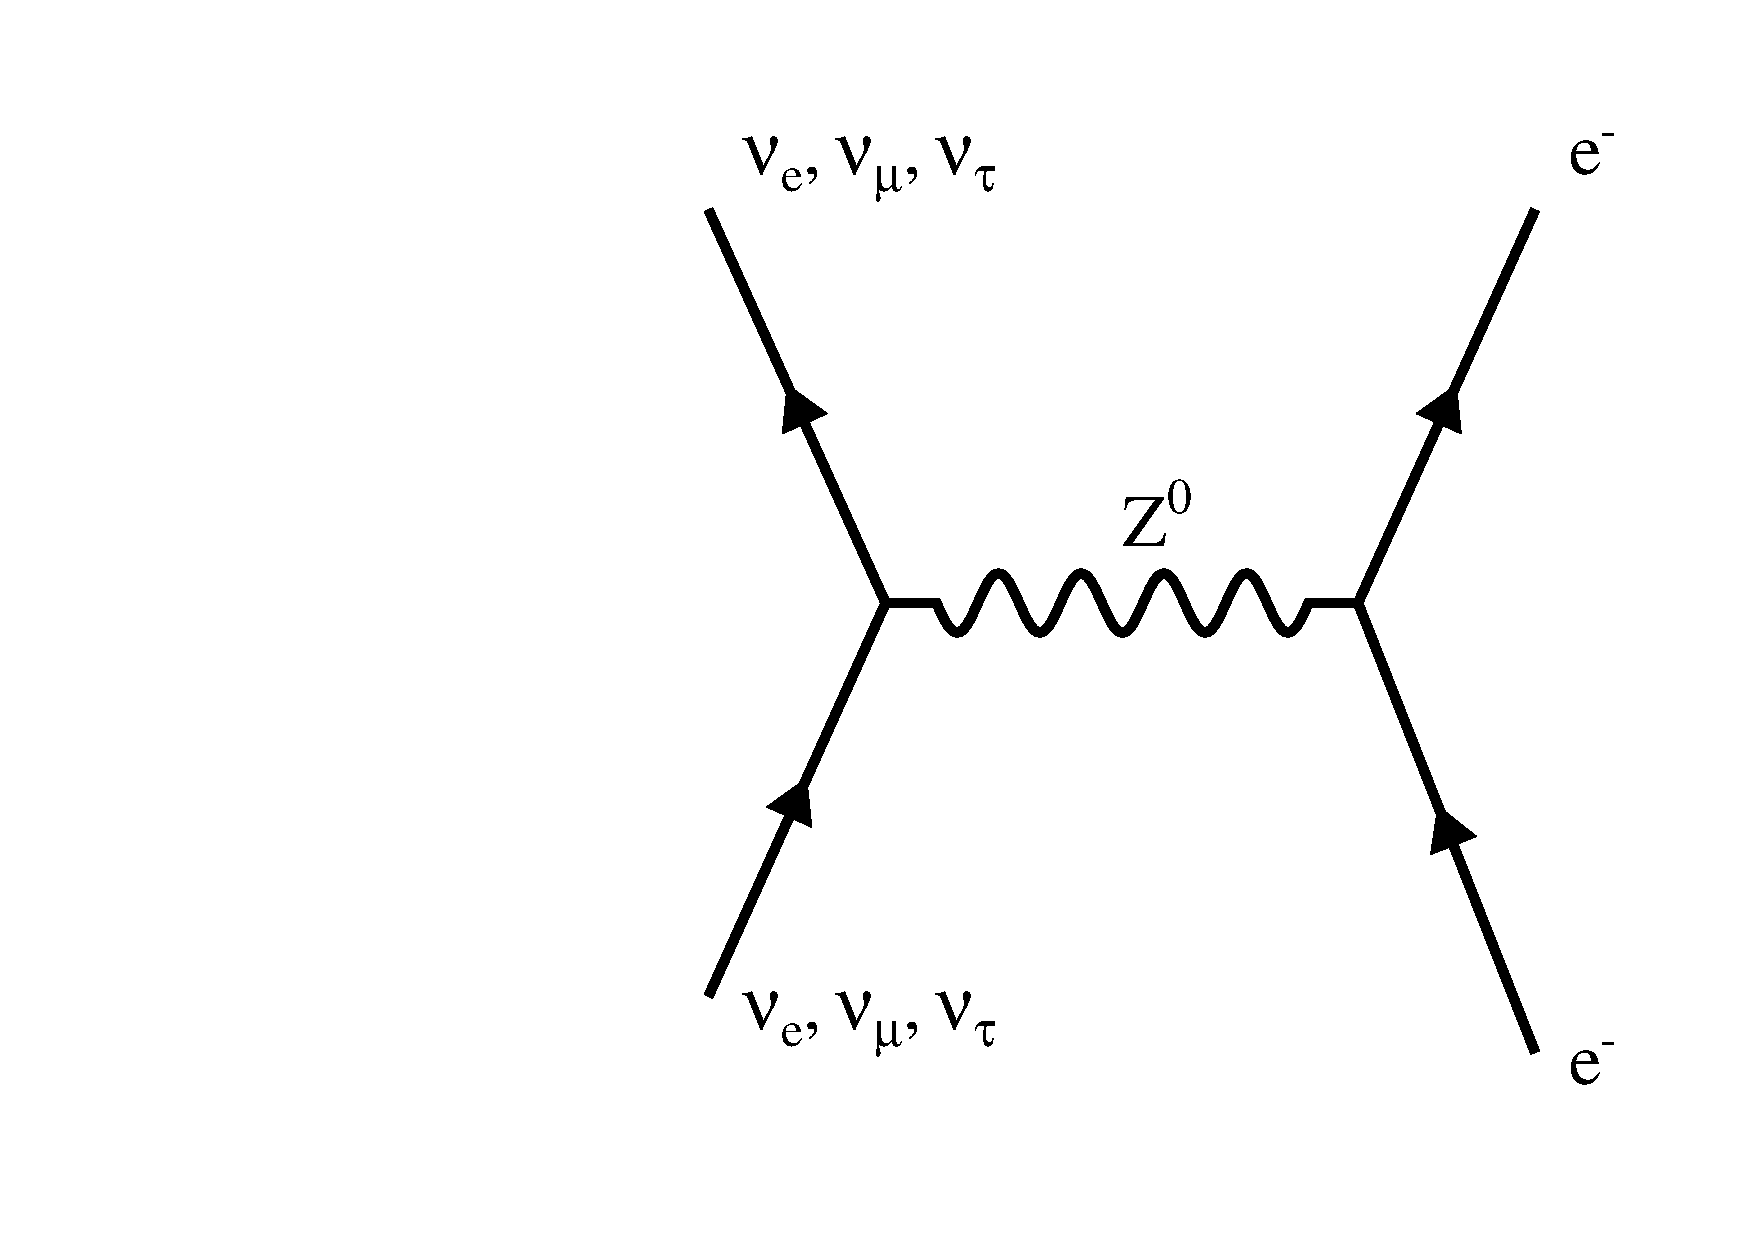
\includegraphics[width=\textwidth]{figures/feynman/ncElec.pdf}
                \caption{}
                 \label{ncElec}
        \end{subfigure}
        ~
\begin{subfigure}[b]{0.3\textwidth}
                \centering
                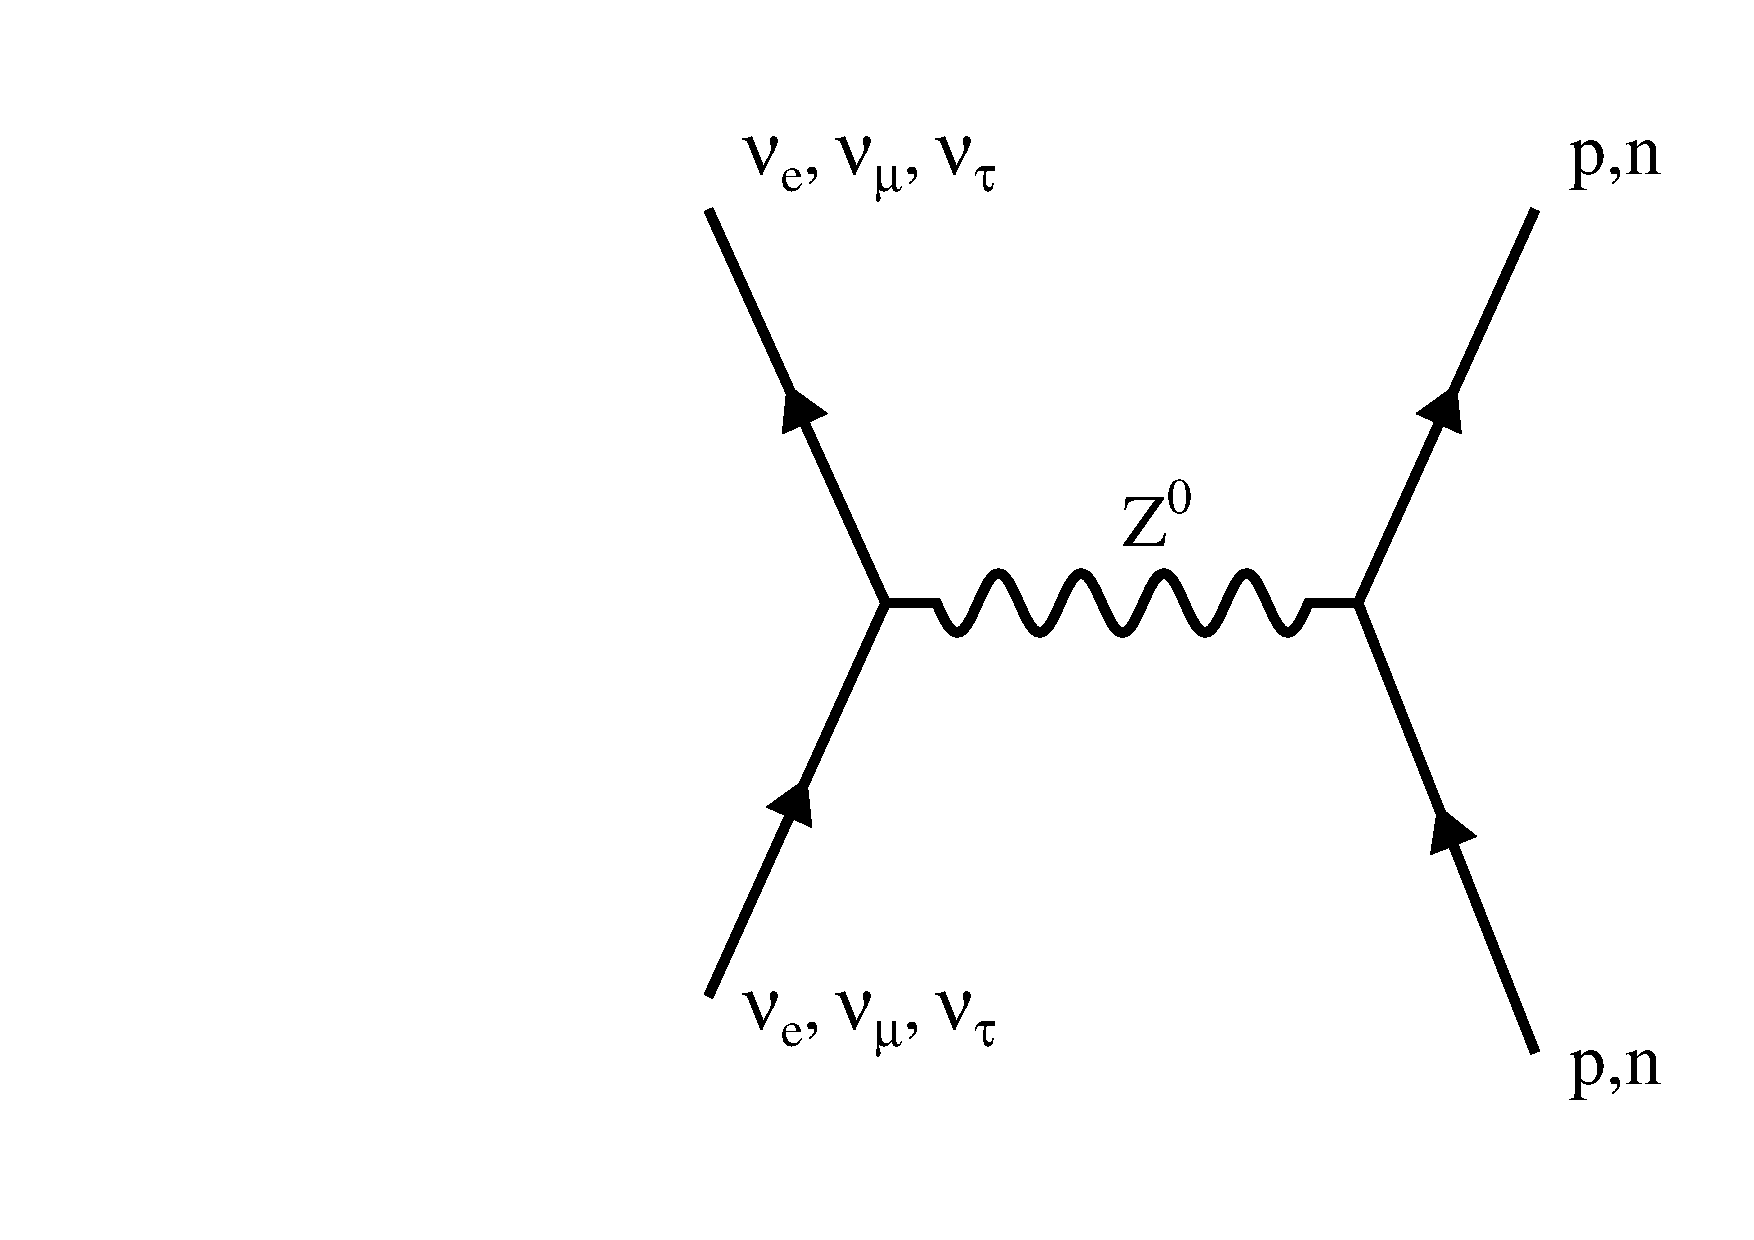
\includegraphics[width=\textwidth]{figures/feynman/ncHad.pdf}
                \caption{}
                 \label{ncHad}
        \end{subfigure}      
        ~
        \begin{subfigure}[b]{0.3\textwidth}
                \centering
                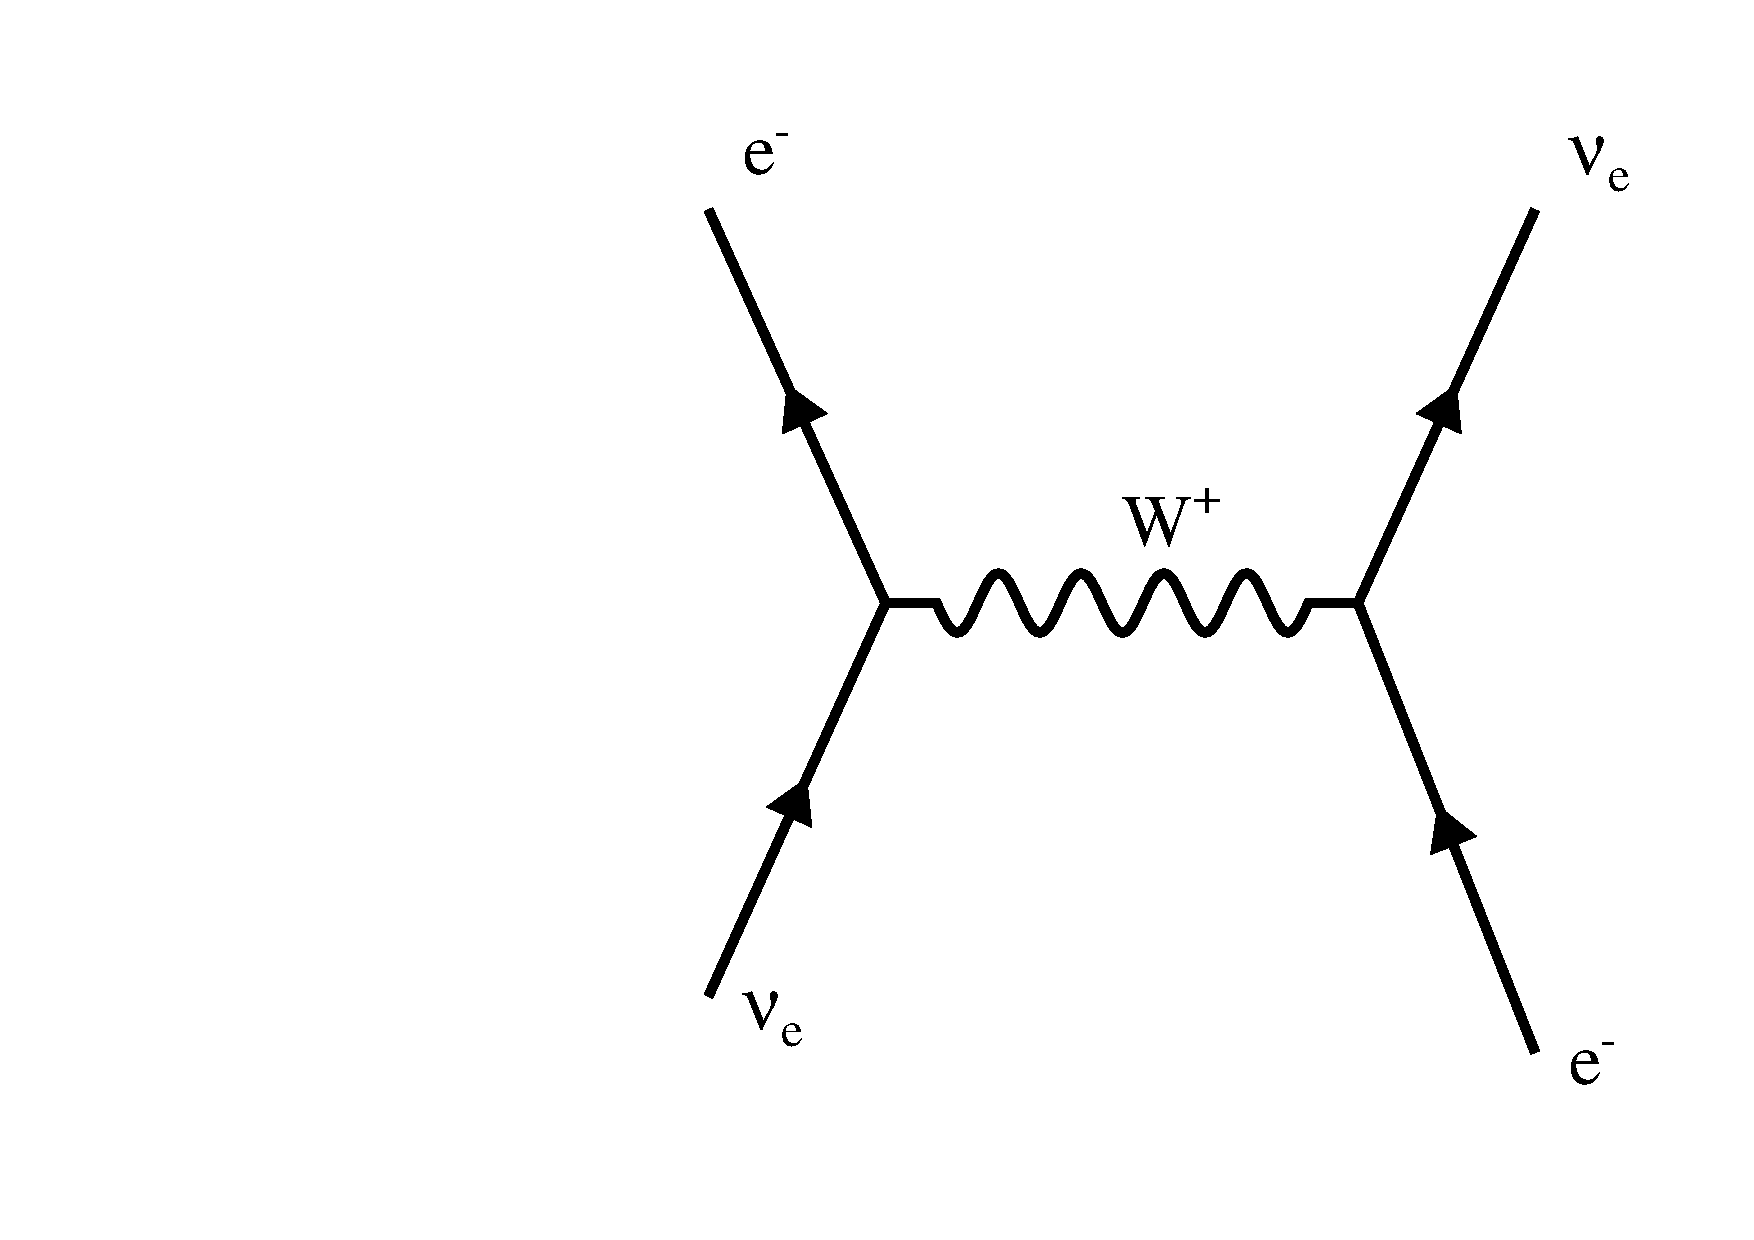
\includegraphics[width=\textwidth]{figures/feynman/ccElec.pdf}
                \caption{}
                 \label{ccElec}
        \end{subfigure}
\caption{Interactions that permit coherent scattering.}
\label{cohScatter}
\end{figure}
A quantitative treatment of this phenomenon imparts particles with an effective mass that modifies their physical mass.  In the case of light, the effective mass manifests itself in the familiar index of refraction that diminishes the speed of light in matter.  For neutrinos, coherent scattering interactions are mediated through the exchange of $W^\pm$ and $Z^0$ bosons; the Feynman diagramsÊfor these interactions can be seen in Figure~\ref{cohScatter}.  The neutral current interactions (those moderated by $Z^0$ exchange) are the same for all three neutrino flavors and have no effectÊon oscillation probabilities.  On the other hand, since terrestrial matter contains electrons but not muons and taus, the charged-current interaction with electrons only occurs for \nue, giving rise to an effective potential:
\begin{equation}
\label{veff}
V_{CC} = \sqrt{2}G_F n_e,
\end{equation}
where $n_e$ is the number density of electrons in the medium and $G_F$ is Fermi's constant.  Since this effective potential only exists for electrons, it modifies the oscillation probabilities given in equation \eqref{oscProbL}, specifically changing the $\sin$ term:
\begin{equation}
\label{modSin}
\sin\bigg(\frac{\Delta m_{\alpha\beta}^2}{2E}L\bigg) \rightarrow 
\frac{\Delta m_{\alpha\beta}^2}{\Delta m_{\alpha\beta}^2 \pm E V_{CC}/2} \sin\bigg((\frac{\Delta m_{\alpha\beta}^2}{2E} \pm \frac{EV_{CC}}{2})L \bigg).
\end{equation}
with the $\pm$ corresponding to a difference in sign for neutrinos and antineutrinos.  This effect is known as the Mikheyev-Smirnov-Wolfenstein (MSW) effect.

\section{Recent Experiments and Results}
In the last two decades experimental neutrino physics has turned the corner from an era of discovery to an era of precision.  The field has made this transition through the use of plentiful sources of neutrinos as well as the development of kiloton scale detectors.  Interestingly enough, despite the growth in scale of neutrino experiments, the techniques have remained largely the same as those of the discovery era.  

Reactor neutrino experiments, like that of Cowan and Reines, have become sensitive enough to measure the survival probability for electron antineutrinos, $P(\bar{\nu_e} \rightarrow \bar{\nu_e})$, and the muon neutrino appearance probability $P(\bar{\nu_e} \rightarrow \bar{\nu_\mu})$.  Accelerator neutrino experiments, not unlike the Brookhaven experiment, can now measure similar probabilities for muon neutrinos, namely, $P(\nu_\mu \rightarrow \nu_\mu$) and $P(\nu_\mu \rightarrow \nu_e)$.  In addition to these common sources, a third plentiful source comes in the form of atmospheric neutrinos.  Cosmic-ray protons interacting in the upper atmosphere produce showers of predominantly pions and kaons that then decay into neutrinos.  If a detector can reconstruct the zenith angle of an atmospheric neutrino, it can determine the distance between its creation and interaction points.  Therefore, a detector that can sample all zenith angles in turn samples a wide range of neutrino baselines ranging from the height of the atmosphere up to the diameter of the earth.  

Reactor neutrinos experiments including KamLAND, Daya Bay and RENO aim to observe the same signal as Cowan and Reines, that is, a prompt $e^+/e^-$ annihilation followed by a delayed neutron capture \cite{kamland, dayaBay, reno}.  Modern versions of these detectors are typically comprised of concentric pairs of tanks filled with liquid scintillator.  The inner tanks are designed to be large enough for neutron containment and the outer tanks are used for rejection of cosmic-ray muons.   Atmospheric neutrino detectors like SNO and Super-Kamiokande (Super-K), on the other hand, are typically water Cerenkov detectors.  Small amounts of light are produced when particles pass through a medium with speed faster than the speed of light in that material, analogous to the wake of a boat or the shock cone of a sonic boom; this light is called Cerenkov radiation.  Water, which can act as a medium for producing Cerenkov radiation, serves as a cheaper alternative to liquid scintillator, allowing larger detectors in terms of both mass and volume.  In both the case of liquid scintillator and water Cerenkov detectors, the light is amplified in photomultiplier tubes, then digitized and stored for analysis.  

The mixing angles have now all been measured to be nonzero by measuring either survival or appearance probabilities.  Precise measurements of \thetaot, the ``solar" mixing angle, have been performed by solar neutrino experiments such as SNO and reactor experiments such as KamLAND \cite{sno, kamland, pdg}.   These measurements yield $\theta_{12} \approx 34^\circ$ with about one $1^\circ$ of uncertainty.  The ``atmospheric" mixing angle, \thetatth has been measured as $\sin^2(\theta_{23}) =  0.514^{+0.055}_{-0.056}$ by neutrino observatories such as SNO and Super-Kamiokande (Super-K) as well as long baseline experiments such as MINOS \cite{sno, superK, minos, pdg}.  Most recently, Daya Bay, RENO, MINOS, T2K, and \nova have made measurements of \thetaoth that are not consistent with zero  \cite{dayaBay, reno, minos13, abe2014observation,nova2015nue}.  The PDG best fit gives $\sin^2(2 \theta_{13}) \approx 0.085 \pm 0.005$

Measurements have also been made of the mass-squared differences.  It is known that $\Delta m_{21}^2$ is $(7.53 \pm 0.18) \times 10^{-5}$ eV${}^2$ and that $|\Delta m_{32}^2|$ is much larger at $(2.42 \pm 0.06) \times10^{-3}$ eV${^2}$.  This means that $\nu_1$ and $\nu_2$ could be similar in mass and that $\nu_3$ is relatively disparate in mass.  On the other hand, no measurements have been made regarding the absolute mass scale of neutrinos, it is also possible that $\nu_1$ is very light and that $\nu_2$ is considerably heavier.  A remaining question is the sign of \deltamtht, commonly called the ordering of the mass hierarchy.  In other words, we do not know whether $\nu_3$ is heavier (referred to as a normal hierarchy) or considerably lighter (inverted hierarchy) than its counterparts.  

%%%%%%%%%%%%%%%%%%%%%%%%%%%%%%%%%%%%%%%%%%%%%%%%%%%%%%%%%%%%%%%%%%%%%%%%%%%%%%%%
